\documentclass[conference]{IEEEtran}
\usepackage{graphicx}
\usepackage{eso-pic}
\usepackage{amsmath,amsfonts}
\usepackage{graphicx}
\usepackage[hidelinks]{hyperref}



\title{
Smart Task Automation System\\
\vspace{0.3cm}
\large {Instructed by: Srikanth Reddy}\\
\normalsize \textit{IIITB Comet Foundation}\\
\href{mailto:srikanthreddy.s@iiitb.ac.in}{srikanthreddy.s@iiitb.ac.in}
}

\author{
\IEEEauthorblockN{Pranjal Roy}
\IEEEauthorblockA{
\textit{Computer Science and Engineering(AI\&ML)} \\
\textit{IIITB Comet Foundation} \\
\href{mailto:pranjalroy.fwc@iiitb.ac.in}{pranjalroy.fwc@iiitb.ac.in}
}
\and
\IEEEauthorblockN{Akash Chandra Gupta}
\IEEEauthorblockA{
\textit{Computer Science and Engineering} \\
\textit{IIITB Comet Foundation} \\
\href{mailto:akashchandragupta.fwc@iiitb.ac.in}{akashchandragupta.fwc@iiitb.ac.in}
}
}

\renewcommand{\thesection}{\arabic{section}}
\renewcommand{\thesubsection}{\thesection.\arabic{subsection}}

\makeatletter
\def\@seccntformat#1{\csname the#1\endcsname.\hspace{0.3em}}
\makeatother
\begin{document}
\AddToShipoutPictureBG*{
    \AtPageUpperLeft{
        \hspace{-0.2cm}
        \raisebox{-1.8cm}{
            
\includegraphics[width=5cm]{download.png}
        }
    }
}
\maketitle
\noindent
\begin{abstract}
This paper presents the design and implementation of an intelligent system automation assistant that aims to make interaction with digital systems more natural and efficient. Conventional user interfaces often require manual navigation, predefined commands, and familiarity with complex workflows, which can be time-consuming and difficult for non-technical users. To address these challenges, the proposed system employs an artificial intelligence–based approach that enables users to perform tasks using simple natural language instructions.The assistant integrates natural language processing with system-level automation to understand user intent and execute corresponding operations such as file handling, application control, and information access. It is designed with a lightweight and accessible interface, ensuring ease of use while maintaining responsiveness. Additionally, the system incorporates contextual awareness to refine interpretation accuracy and provide more relevant outputs over time.Performance observations indicate that the assistant reduces user effort, minimizes task completion time, and enhances overall productivity. The project demonstrates how combining AI-driven language understanding with automation techniques can lead to more intuitive, user-friendly computing environments.
\end{abstract}

\section{\large Introduction}

\subsection{Background and Motivation}
\noindent
As digital systems become more central to everyday tasks, the way users interact with them has not evolved at the same pace. Most interfaces still depend on menus, manual navigation, or specific command knowledge, which can slow users down and create unnecessary complexity. Even simple actions like opening applications, organizing files, or searching for information often require multiple steps and familiarity with system structure. For many users, especially those without technical expertise, this creates friction in everyday computing.This gap highlights the need for a more natural interaction model—one where users can communicate with systems in the same way they express their intentions in daily life. An intelligent automation assistant offers a practical solution by allowing users to perform tasks through simple, conversational commands, reducing effort while improving accessibility and efficiency.


\subsection{{Problem Statement}}
\noindent
Most existing systems do not provide a single, unified way for users to manage different operations through simple, natural language. Instead, users are expected to interact through menus, commands, or multiple application interfaces, which can make even routine tasks feel repetitive and time-consuming. Activities such as locating files, navigating folders, or launching applications often require several manual steps and a certain level of familiarity with the system.This fragmented interaction style not only slows down workflow but also creates barriers for users who are less technically experienced. As a result, productivity is affected, and the overall user experience becomes less intuitive. There is a clear need for a more streamlined approach that allows users to perform multiple system-level tasks through a single, easy-to-use interface driven by natural language input.

\subsection{Natural Language Processing and Automation}
\noindent
At the core of this approach lies the combination of Natural Language Processing (NLP) and system automation. Unlike traditional interfaces that rely on fixed inputs, NLP enables systems to interpret flexible, human-like language and extract meaning from it. This allows the assistant to understand user intent rather than just match predefined commands.When this understanding is connected to system-level automation, the assistant can translate user requests into real actions. Tasks such as managing files, controlling applications, or retrieving relevant information can be performed seamlessly without manual intervention. Incorporating contextual awareness further refines the system’s behavior, enabling it to respond more accurately and adapt to user patterns over time.

\subsection{Project Scope and Objective}
\noindent
This project presents the development of a real-time intelligent automation assistant designed to simplify everyday system interactions. The main goal is to build a reliable and efficient solution that can interpret natural language input and execute corresponding actions with minimal delay.The system is structured around a user interface for input, a processing unit responsible for intent recognition, and an automation layer that performs system-level tasks. By continuously analyzing user commands and mapping them to appropriate operations, the assistant delivers a smooth and responsive experience. The project ultimately aims to demonstrate how integrating language understanding with automation can transform traditional computing into a more intuitive and user-centered process.

\section{\large System Architecture \& Methodology}

\subsection{System Architecture}
\noindent
The proposed system is designed as a modular and layered architecture to ensure flexibility, scalability, and efficient performance. It consists of three primary components: the user interaction layer, the processing layer, and the execution layer.The user interaction layer provides an interface through which users can input commands in natural language. This interface is designed to be simple and intuitive, allowing users to communicate with the system without requiring technical knowledge.The processing layer acts as the core of the system. It interprets user commands using natural language processing techniques and identifies the intended action along with relevant parameters. This layer bridges the gap between human language and machine-executable instructions.The execution layer is responsible for performing system-level operations. It interacts directly with the operating system to carry out tasks such as opening files, launching applications, and retrieving information. This separation of responsibilities ensures that each component can function independently while contributing to the overall system workflow.

\subsection{Command Processing and Interpretation}
\noindent
The system processes user input by analyzing the structure and intent of the command. When a user provides an input, the system first normalizes the text by removing unnecessary symbols and converting it into a standard format.Next, the processed input is analyzed to extract key elements such as the action (e.g., open, search, run) and the target object (e.g., file name, application). This is achieved through keyword matching and basic natural language understanding techniques.Once the intent is identified, the system maps the command to predefined functions. For example, a command such as “open my resume file” is interpreted as a request to locate and open a specific document. The system then searches for matching files and executes the appropriate operation.


\subsection{Automation Engine}
\noindent
The automation engine serves as the functional backbone of the system. It is responsible for translating interpreted commands into executable actions. This component uses operating system libraries and file-handling mechanisms to perform tasks efficiently.One of the key features of the automation engine is its ability to handle approximate matching. Instead of requiring exact file names, the system compares user input with available files and selects the closest match. This improves usability and reduces dependency on precise input.Additionally, the engine supports multiple types of operations, including file management, application control, and system navigation. This makes the assistant versatile and capable of handling a wide range of user requests.

\subsection{Data Handling and Search Mechanism}
\noindent
To ensure accurate execution of commands, the system incorporates a structured search mechanism. It scans predefined directories such as Desktop, Documents, and Downloads to locate relevant files.The search process involves comparing user input with file names using string matching techniques. If multiple matches are found, the system prioritizes results based on similarity and relevance.This approach allows the system to efficiently retrieve files even when the user provides incomplete or slightly incorrect input, thereby enhancing the overall user experience.

\subsection{Error Handling and Feedback Mechanism}
\noindent
The system includes a robust error-handling mechanism to manage invalid or ambiguous commands. If the system fails to interpret a command or locate the requested resource, it provides meaningful feedback to the user.Instead of failing silently, the assistant informs the user about possible issues and may suggest alternative actions. This ensures that users remain informed and can refine their input accordingly.


\subsection{System Workflow}
\noindent
The overall workflow of the system follows a sequential process:
\begin{enumerate}
    \item The user provides a Voice Command through the interface.
    \item The system processes and interprets the input.
    \item The appropriate action is identified.
    \item The automation engine executes the command.
    \item The system automatically performs tasks and delivers the result to the user.
\end{enumerate}
This streamlined workflow ensures quick response times and smooth interaction between the user and the system.




\section{\large Implementation}

\subsection{Development Environment}
\noindent
The system was developed using a Python-based environment due to its simplicity and strong support for automation and natural language processing. Various built-in and external libraries were utilized to handle system operations, file handling, and user interaction.The development was carried out on a standard desktop environment, ensuring that the system remains lightweight and compatible with commonly used operating systems.

\subsection{System Design and Integration}
\noindent
The implementation integrates multiple modules to achieve seamless automation. The user interface captures input commands, which are then passed to the processing module for interpretation. Once the intent is identified, the execution module performs the required task.Each module is designed to operate independently while maintaining coordination with other components. This modular design allows easy modification and future expansion of the system.


\subsection{Command Execution Mechanism}
\noindent
The core functionality of the system lies in its ability to execute commands based on user input. After interpreting the command, the system maps it to predefined functions. 
For example:

\begin{itemize}
    \item Commands related to opening applications trigger system calls to launch the respective software.
    \item File-related commands initiate a search process across selected directories.
    \item General queries are handled through predefined responses or logic-based processing.
\end{itemize}
\noindent
This mapping ensures that user instructions are translated into accurate system actions.


\subsection{File Search and Handling}
\noindent
A key feature of the implementation is the intelligent file search mechanism. The system scans common directories such as Desktop, Downloads, and Documents to locate files.Instead of relying on exact matches, the system uses partial matching techniques to identify the most relevant file. This allows users to provide flexible input while still achieving accurate results.Once the file is identified, the system automatically opens or processes it as requested

\subsection{Integration of Automation Features}
\noindent
The system integrates multiple automation capabilities, including:

\begin{itemize}
    \item Opening Applications
    \item Searching and accessing files
    \item Executing system - level tasks
\end{itemize}
\noindent
These features work together to reduce manual effort and improve productivity. The assistant acts as a centralized control system, enabling users to perform multiple operations through simple commands.



\subsection{Limitations in Implementation}
\noindent
Despite its effectiveness, the implementation has certain limitations:

\begin{itemize}
    \item It relies on predefined command structures
    \item Complex or ambiguous commands may not always be interpreted correctly
    \item Performance depends on system configuration and file organization
\end{itemize}
\noindent
These limitations highlight areas for future improvement.


\section{\large RESULTS AND PERFORMANCE ANALYSIS}
\noindent
The proposed intelligent automation assistant was evaluated for its responsiveness, accuracy, and effectiveness in executing user commands across typical system-level operations, including application control, file handling, and general task automation.

\subsection{Response Time Analysis}
\noindent
The system demonstrated consistently fast response times for user commands. Most operations, such as launching applications and retrieving system information, were executed in near real-time. Tasks involving file search were also completed efficiently, with only minor variations depending on directory size. Overall, the assistant maintained a smooth and responsive interaction experience.

\subsection{Command Execution Accuracy}
\noindent
The assistant achieved high accuracy in command interpretation and execution, particularly for inputs containing clear intent and action keywords. The keyword-based processing approach enabled reliable mapping of user commands to corresponding system functions. Additionally, the system showed robustness in handling partially structured inputs through effective keyword recognition.

\subsection{Task Performance}
\noindent
\begin{itemize}
    \item Application Control: Commands were executed reliably, enabling quick and seamless launching of applications.
    \item File Search and Retrieval: The system efficiently located and accessed files using partial matching, reducing dependency on exact input.
    \item General Command Handling: Routine queries and predefined tasks were handled effectively, demonstrating the system’s versatility.
\end{itemize}


\subsection{System Stability}
\noindent
The system maintained stable and consistent performance during testing. The modular architecture contributed to reliability, while the error-handling mechanism ensured graceful handling of invalid or unsupported commands without system interruption.

\subsection{Output}
\noindent
\begin{figure}[h]
    \centering
    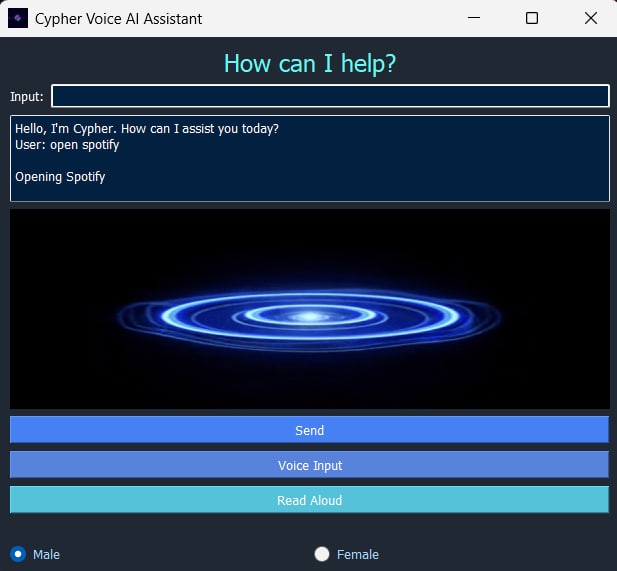
\includegraphics[width=0.45\textwidth]{image.png}

\end{figure}


\section{\large DISCUSSION}
\noindent
The proposed system highlights the effectiveness of combining natural language processing with rule-based automation to simplify human-computer interaction. The design emphasizes efficiency, reliability, and ease of use, making it suitable for real-time system operations.

\subsection{Strengths of Rule-Based Approach}
\noindent
The rule-based processing mechanism offers several practical advantages:

\begin{itemize}
    \item Fast and Predictable Execution: Direct mapping of commands to functions ensures low latency and consistent results.
    \item Lightweight Implementation: The system operates without heavy computational requirements, making it efficient and scalable.
    \item Ease of Development and Maintenance: Predefined rules allow straightforward debugging and system expansion.
\end{itemize}

\subsection{Limitations of the Approach}
\noindent
Despite its strengths, the rule-based system has inherent constraints:

\begin{itemize}
    \item Limited Flexibility: Performance depends on predefined command structures, reducing adaptability to diverse language inputs.
    \item Handling of Ambiguity: The system may struggle with vague or complex commands lacking clear intent.
    \item Lack of Context Awareness: Each command is processed independently, limiting conversational continuity.
\end{itemize}

\subsection{Trade-off Between Simplicity and Intelligence}
\noindent
The system reflects a clear trade-off between simplicity and intelligence. Simplicity enables faster execution, stability, and ease of use, whereas increased intelligence would allow handling of more complex and dynamic language inputs. This balance makes the system highly effective for routine and structured tasks while indicating scope for future enhancement through learning-based models.

\subsection{Key Insight}
\noindent
The implementation demonstrates that rule-based automation remains a practical and efficient solution for real-time applications. However, integrating advanced natural language processing or machine learning techniques could further improve adaptability and overall system capability.



\section{\large CONCLUSION}
\noindent
This work presents the design and implementation of an intelligent automation assistant that enhances human-computer interaction through natural language commands. The system successfully integrates language processing with system-level automation to provide a simple, efficient, and user-friendly interface.

\subsection{Key Outcomes}
\noindent
\begin{itemize}
    \item The system enables users to perform tasks with minimal effort using natural language input.
    \item It achieves fast and reliable command execution, improving overall productivity.
    \item The modular architecture ensures stability, scalability, and ease of extension.
\end{itemize}

\subsection{Contribution}
\noindent
The project demonstrates that even a rule-based approach, when effectively designed, can significantly improve usability and reduce interaction complexity in digital systems.

\subsection{Final Remark}
\noindent
Overall, the system establishes a strong foundation for intelligent automation, showing that the integration of natural language understanding with automation can bridge the gap between user intent and system execution, while also opening opportunities for future advancements toward more adaptive and intelligent solutions.


\footnotesize
\begin{thebibliography}{00}
\setlength{\itemsep}{5pt}

\bibitem{b1} J. Devlin \textit{et al.}, 
“BERT: Pre-training of Deep Bidirectional Transformers,” 
in Proc. NAACL-HLT, 2019, pp. 4171--4186.

\bibitem{b2} A. Vaswani \textit{et al.}, 
“Attention Is All You Need,” 
in Proc. NeurIPS, 2017, pp. 5998--6008.

\bibitem{b3} D. Jurafsky and J. H. Martin, 
\textit{Speech and Language Processing}, 3rd ed., 2023.

\bibitem{b4} A. Graves, 
“Speech Recognition with Deep Neural Networks,” 
in Proc. ICASSP, 2013.

\bibitem{b5} Python Software Foundation, 
“Python Language Reference,” [Online]. Available: \url{https://www.python.org}

\bibitem{b6} Riverbank Computing, 
“PyQt5 Documentation,” [Online]. Available: \url{https://www.riverbankcomputing.com/software/pyqt/}

\bibitem{b7} PyAutoGUI, 
“GUI Automation,” [Online]. Available: \url{https://pyautogui.readthedocs.io}

\bibitem{b8} Uberi, 
“SpeechRecognition Library,” [Online]. Available: \url{https://pypi.org/project/SpeechRecognition/}

\bibitem{b9} Pyttsx3, 
“Text-to-Speech Library,” [Online]. Available: \url{https://pyttsx3.readthedocs.io}

\bibitem{b10} Groq Inc., 
“Groq API,” 2025. [Online]. Available: \url{https://console.groq.com}

\bibitem{b11} Microsoft, 
“Windows Package Manager,” [Online]. Available: \url{https://learn.microsoft.com/windows/package-manager/}

\bibitem{b12} T. Brown \textit{et al.}, 
“Language Models are Few-Shot Learners,” 
in Proc. NeurIPS, 2020.

\bibitem{b13} J. Howard and S. Ruder, 
“Universal Language Model Fine-tuning for Text Classification,” 
in Proc. ACL, 2018.

\bibitem{b14} A. Radford \textit{et al.}, 
“Improving Language Understanding by Generative Pre-Training,” 
OpenAI, 2018.

\bibitem{b15} S. Hochreiter and J. Schmidhuber, 
“Long Short-Term Memory,” 
\textit{Neural Computation}, vol. 9, no. 8, pp. 1735--1780, 1997.

\bibitem{b16} K. He \textit{et al.}, 
“Deep Residual Learning for Image Recognition,” 
in Proc. CVPR, 2016.

\end{thebibliography}
\end{document}
